% Created 2021-05-16 Sun 18:25
% Intended LaTeX compiler: pdflatex
\documentclass[presentation]{beamer}
\usepackage[utf8]{inputenc}
\usepackage[T1]{fontenc}
\usepackage{graphicx}
\usepackage{grffile}
\usepackage{longtable}
\usepackage{wrapfig}
\usepackage{rotating}
\usepackage[normalem]{ulem}
\usepackage{amsmath}
\usepackage{textcomp}
\usepackage{amssymb}
\usepackage{capt-of}
\usepackage{hyperref}
\usetheme{Warsaw}
\author{\href{mailto:lorenzo.lastrucci@mail.polimi.it}{Lorenzo Lastrucci}, \href{mailto:daniele.paletti@mail.polimi.it}{Daniele Paletti}}
\date{2021-05-04}
\title{State of MIDA-ACV Project}
\institute[Politecnico di Milano]{Politecnico di Milano}
\titlegraphic{\includegraphics[height=1.5cm]{/home/dpaletti/Pictures/polimi.png}}
\AtBeginSection{\frame{\sectionpage}}
\usepackage{booktabs}
\usecolortheme{seahorse}
\setbeamertemplate{headline}{}
\usepackage{tikz}
\usetikzlibrary{snakes}
\usepackage{rotating}
\hypersetup{
 pdfauthor={\href{mailto:lorenzo.lastrucci@mail.polimi.it}{Lorenzo Lastrucci}, \href{mailto:daniele.paletti@mail.polimi.it}{Daniele Paletti}},
 pdftitle={State of MIDA-ACV Project},
 pdfkeywords={},
 pdfsubject={},
 pdfcreator={Emacs 27.2 (Org mode 9.5)}, 
 pdflang={English}}
\begin{document}

\maketitle

\section{Data Exploration}
\label{sec:orgbfebfc1}
\begin{frame}[label={sec:org040ff2d}]{Scooter Path}
\begin{figure}[htbp]
\centering
\includegraphics[width=.9\linewidth]{/home/dpaletti/Pictures/path_giovanni_coral_red.png}
\caption{\label{fig:path_giovanni_coral}Path from Coral's Run (stem recording)}
\end{figure}
\end{frame}
\begin{frame}[label={sec:org429417e}]{Speed: one driver, low weight}
\begin{figure}[htbp]
\centering
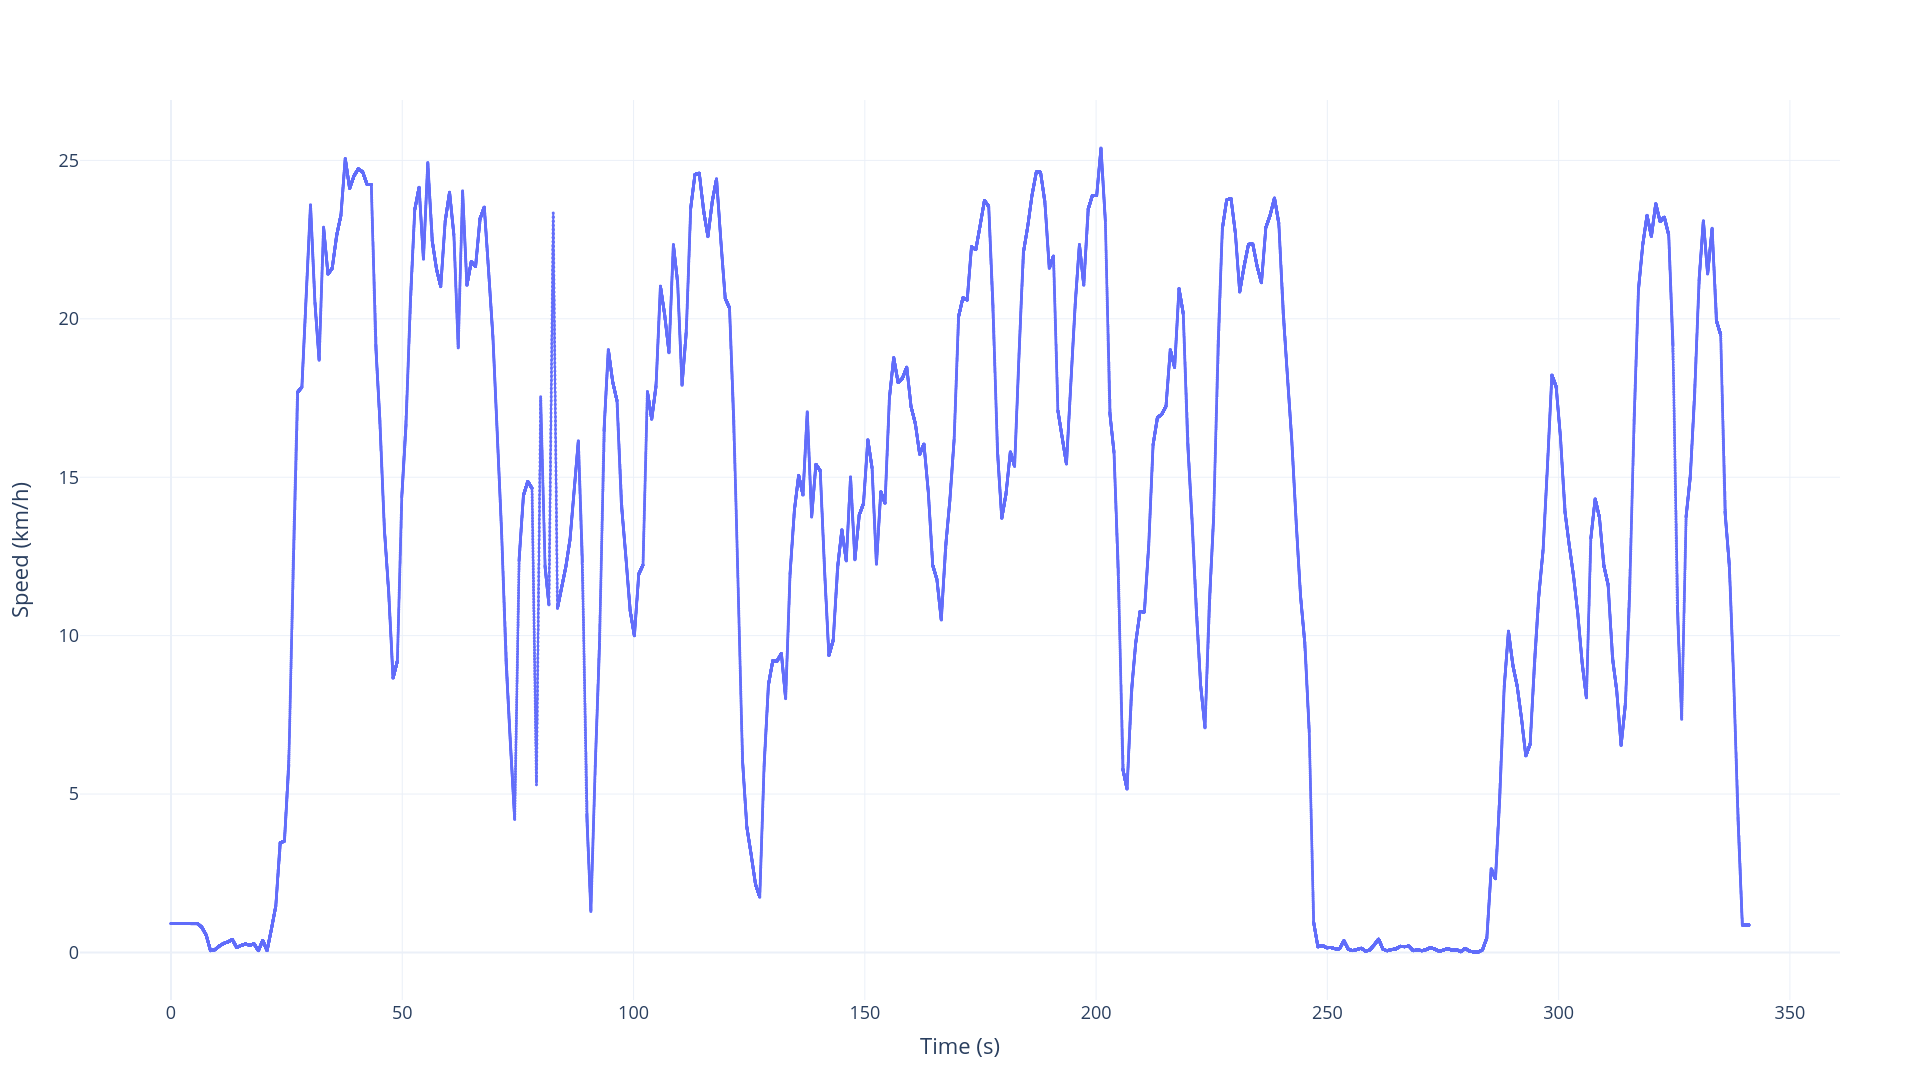
\includegraphics[width=.9\linewidth]{/home/dpaletti/mida_acv/resources/plots/speed_full_leoni_35.png}
\caption{\label{fig:speed_jessica}Speed from Leoni's recording}
\end{figure}
\end{frame}
\begin{frame}[label={sec:org4efab1e}]{Speed: one driver, high weight}
\begin{figure}[htbp]
\centering
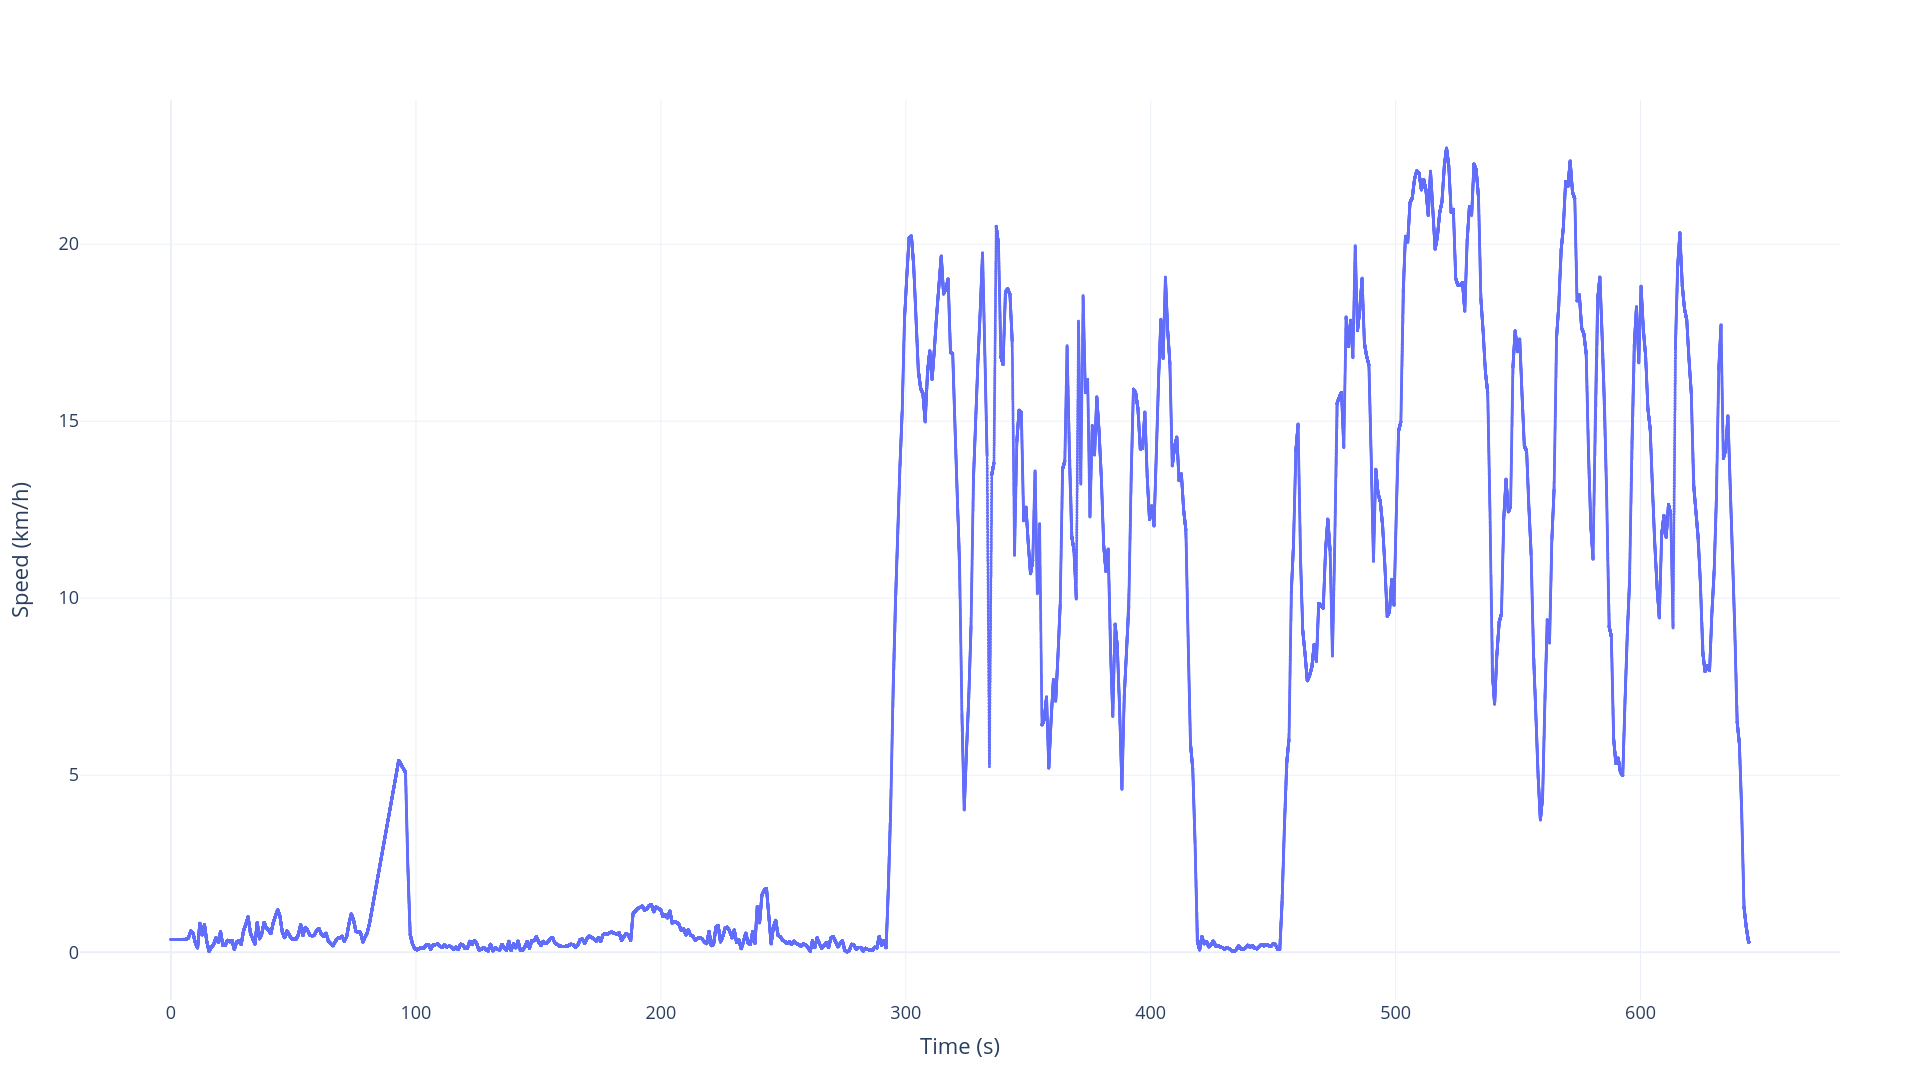
\includegraphics[width=.9\linewidth]{/home/dpaletti/mida_acv/resources/plots/speed_full_didonato_105.png}
\caption{\label{fig:speed_jessica}Speed from Didonato's recording}
\end{figure}
\end{frame}

\begin{frame}[label={sec:orgaf0cf35}]{Speed: two drivers}
\begin{figure}[htbp]
\centering
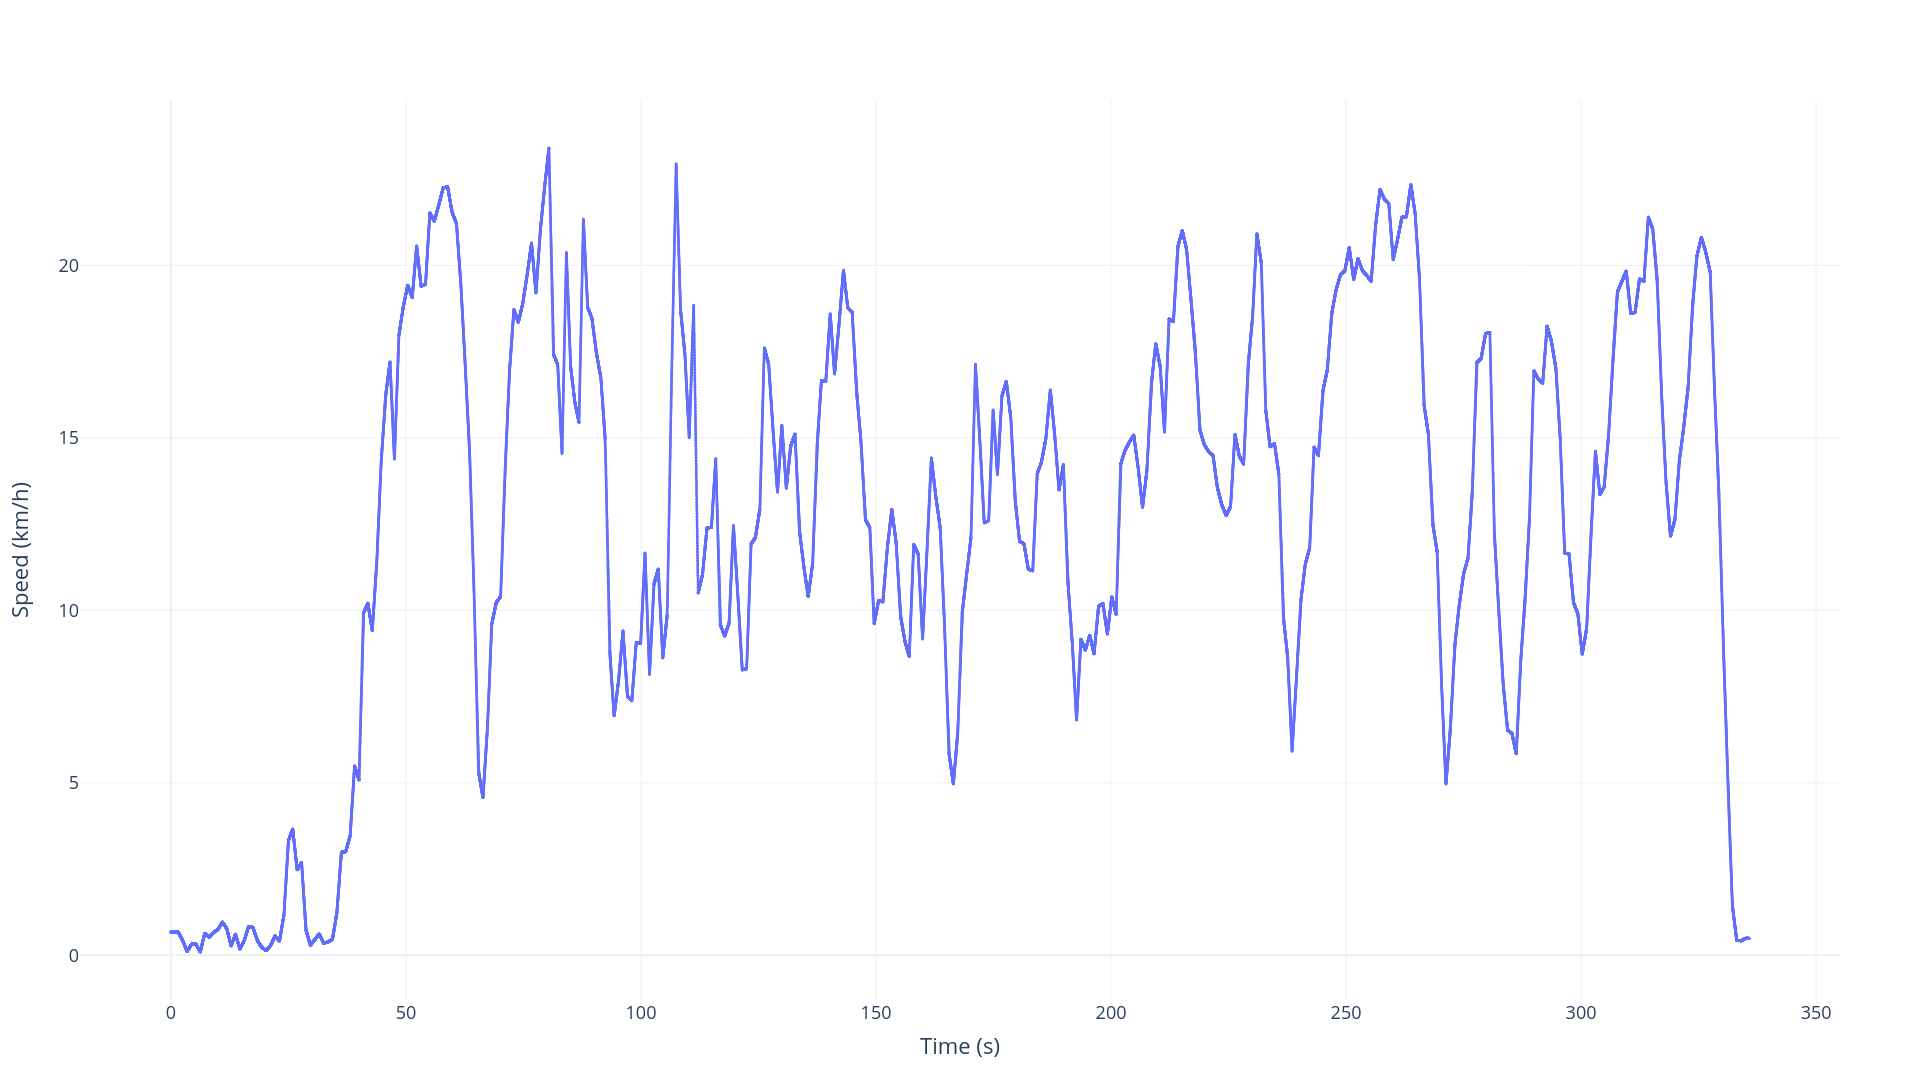
\includegraphics[width=.9\linewidth]{/home/dpaletti/mida_acv/resources/plots/speed_full_alberto_jessica_108.png}
\caption{\label{fig:speed_alberto_jessica}Speed from Didonato and Leoni's recording}
\end{figure}
\end{frame}
\begin{frame}[label={sec:org04bd422}]{Acceleration: one driver, low weight}
\begin{figure}[htbp]
\centering
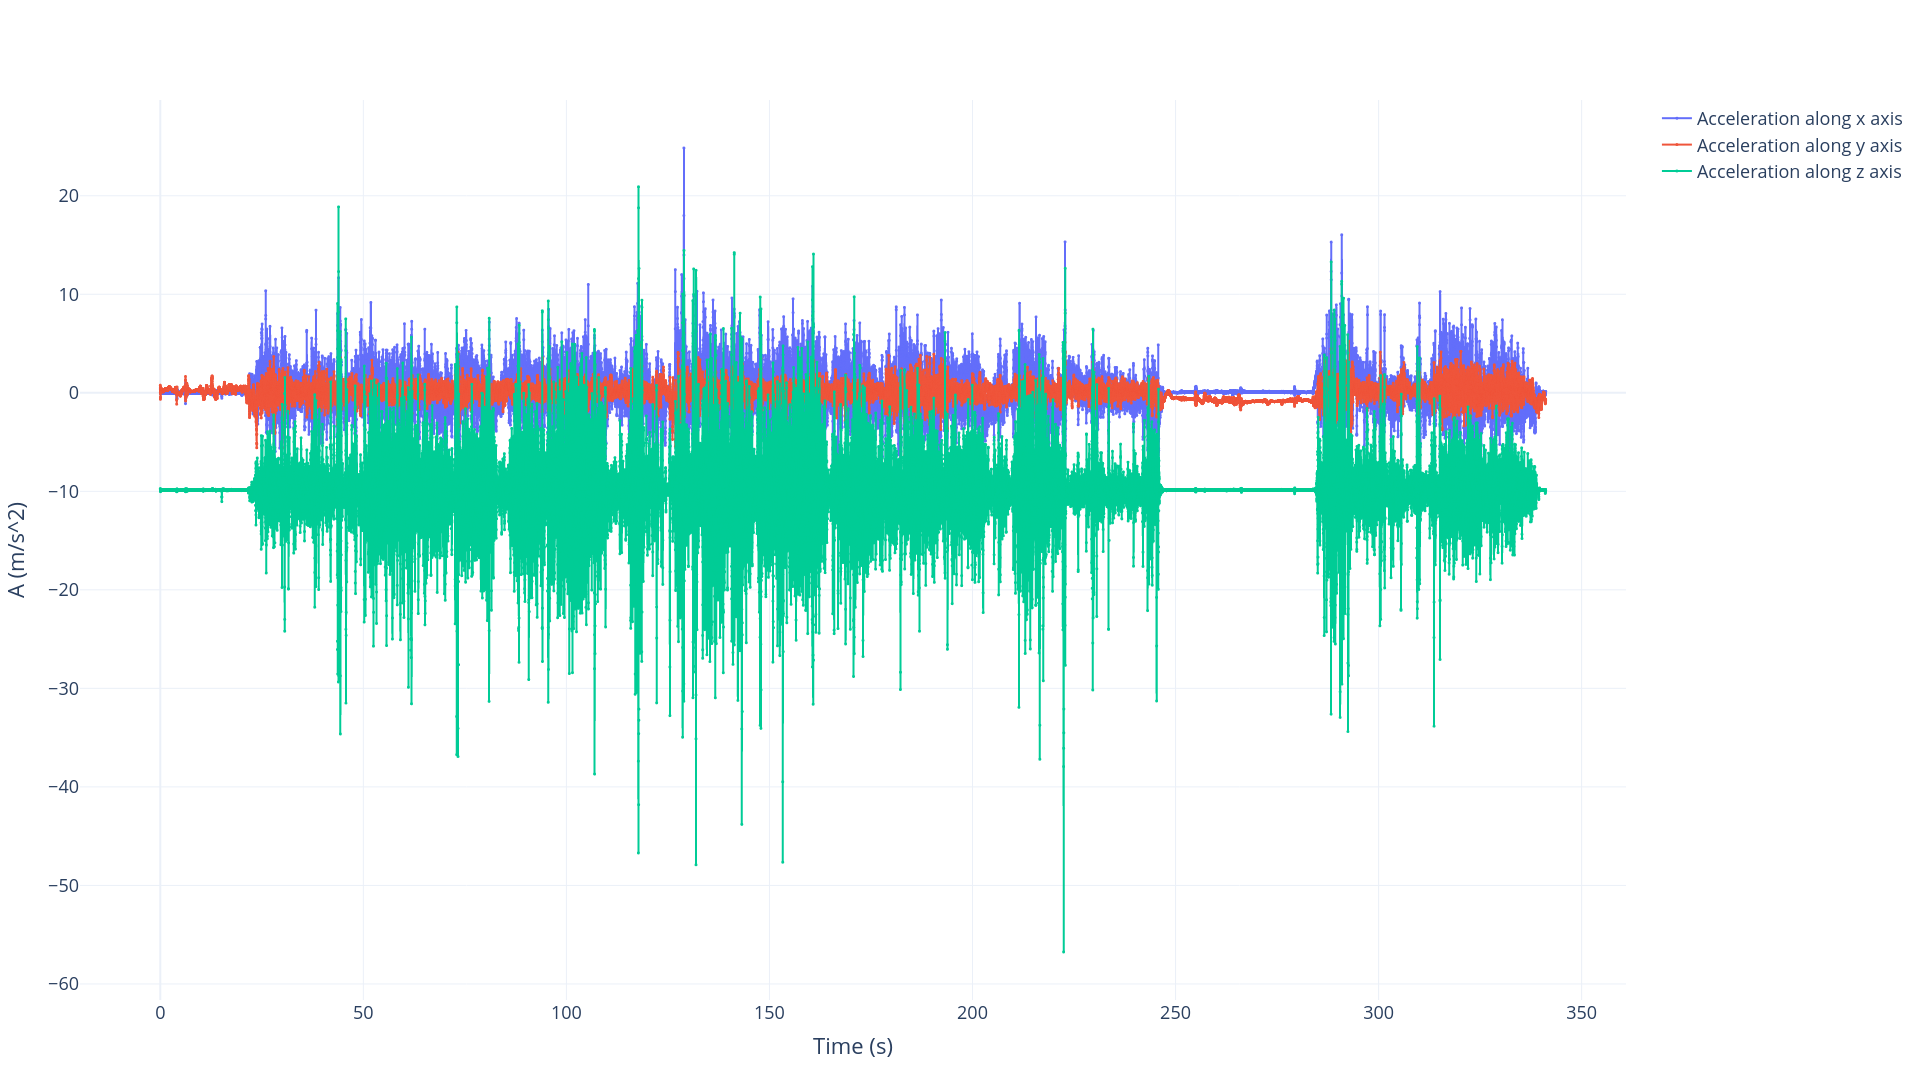
\includegraphics[width=.9\linewidth]{/home/dpaletti/mida_acv/resources/plots/acceleration_full_leoni_35.png}
\caption{\label{fig:speed_jessica}Acceleration from Leoni's recording}
\end{figure}
\end{frame}
\begin{frame}[label={sec:org5415cc9}]{Acceleration: one driver, high weight}
\begin{figure}[htbp]
\centering
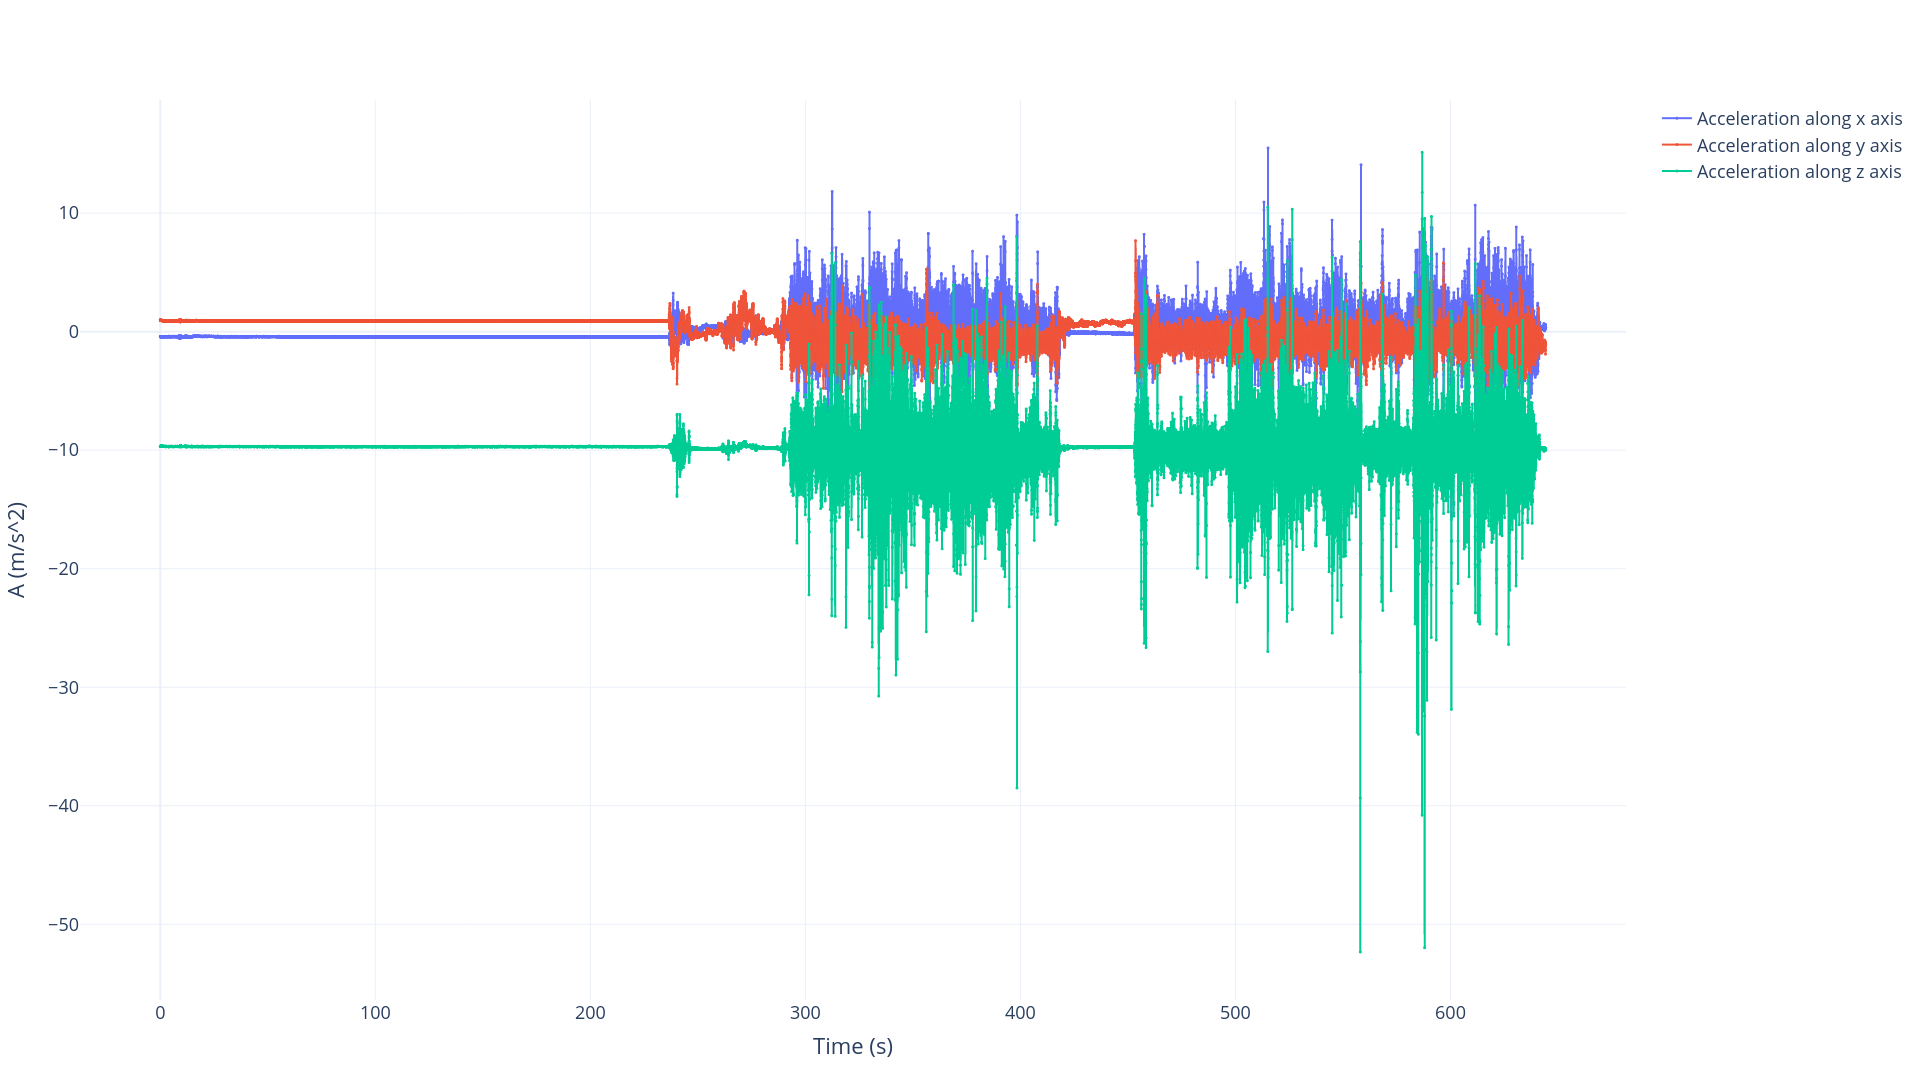
\includegraphics[width=.9\linewidth]{/home/dpaletti/mida_acv/resources/plots/acceleration_full_didonato_105.png}
\caption{\label{fig:speed_jessica}Acceleration from Didonato's recording}
\end{figure}
\end{frame}
\begin{frame}[label={sec:orgaed43bc}]{Acceleration: two drivers}
\begin{figure}[htbp]
\centering
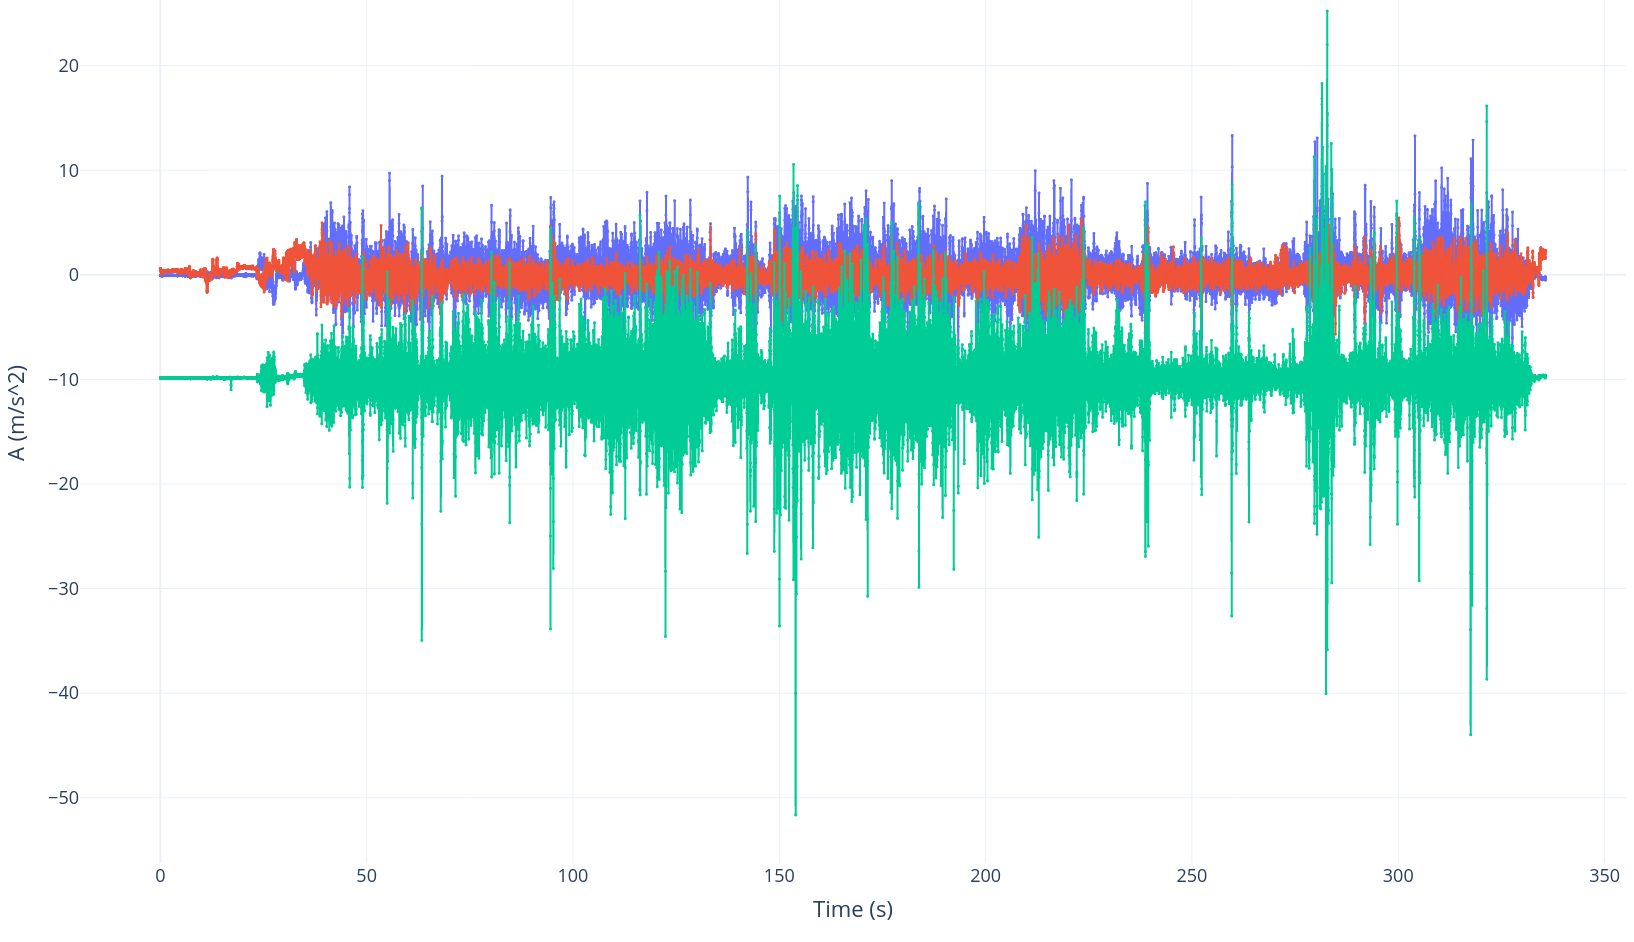
\includegraphics[width=.9\linewidth]{/home/dpaletti/mida_acv/resources/plots/acceleration_full_alberto_jessica_108.png}
\caption{\label{fig:speed_alberto_jessica}Acceleration from Didonato and Leoni's recording}
\end{figure}
\end{frame}

\begin{frame}[label={sec:org9ed5c3f}]{Jerk: one driver, low weight}
\begin{figure}[htbp]
\centering
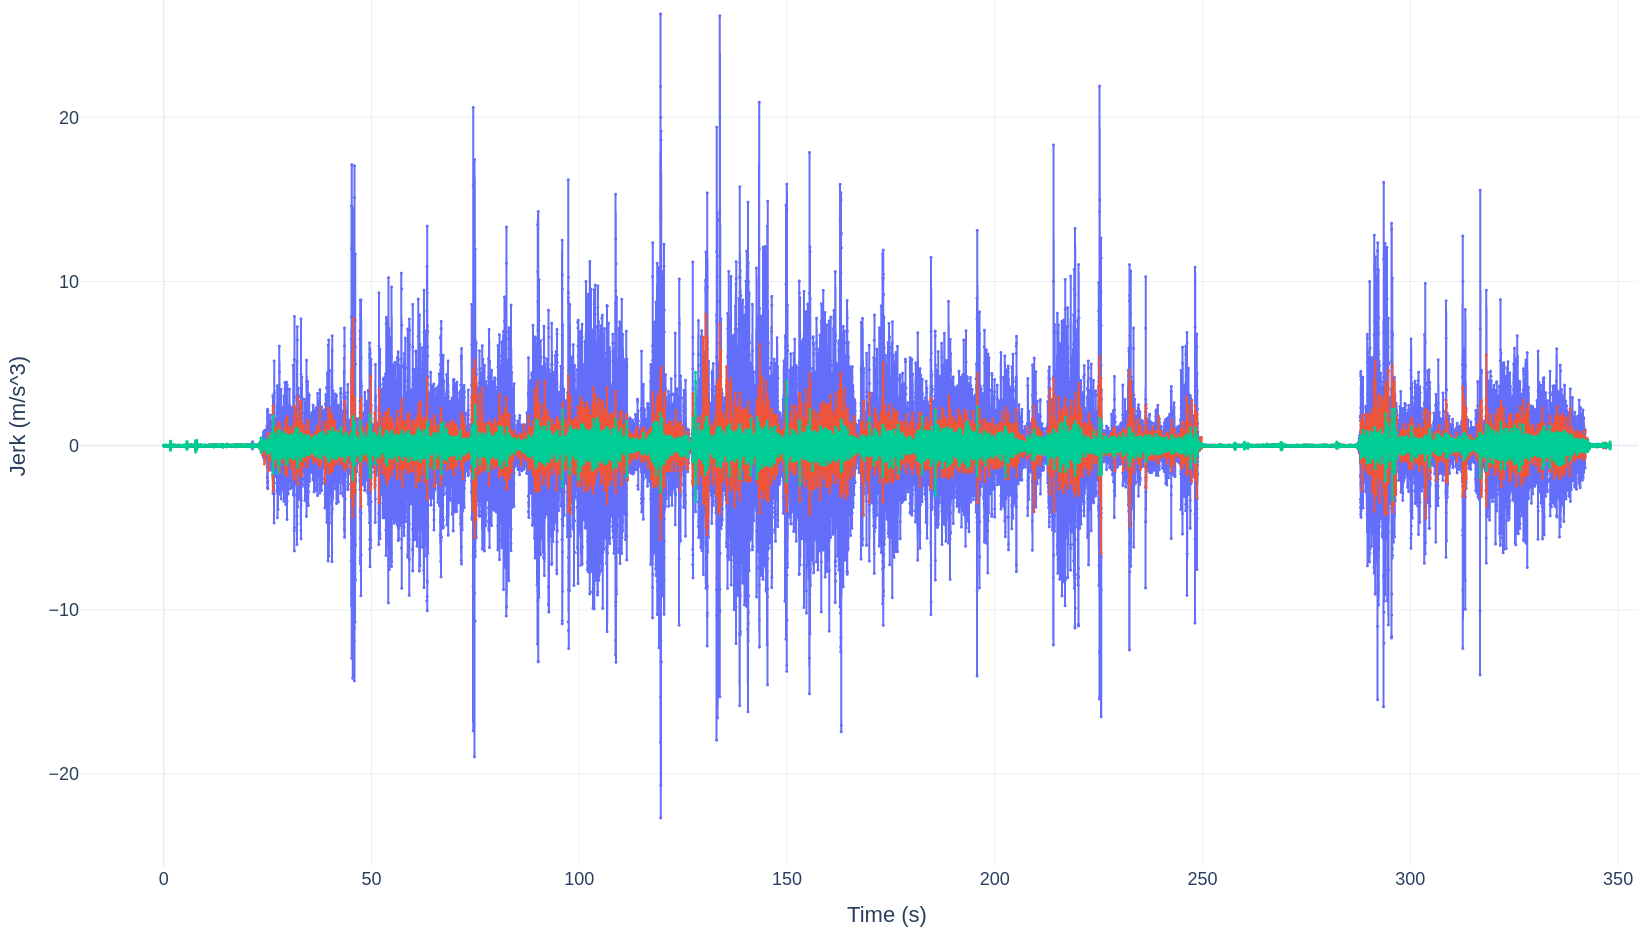
\includegraphics[width=.9\linewidth]{/home/dpaletti/mida_acv/resources/plots/jerk_full_leoni_35.png}
\caption{\label{fig:speed_jessica}Jerk from Leoni's recording}
\end{figure}
\end{frame}
\begin{frame}[label={sec:org20782c6}]{Jerk: one driver, high weight}
\begin{figure}[htbp]
\centering
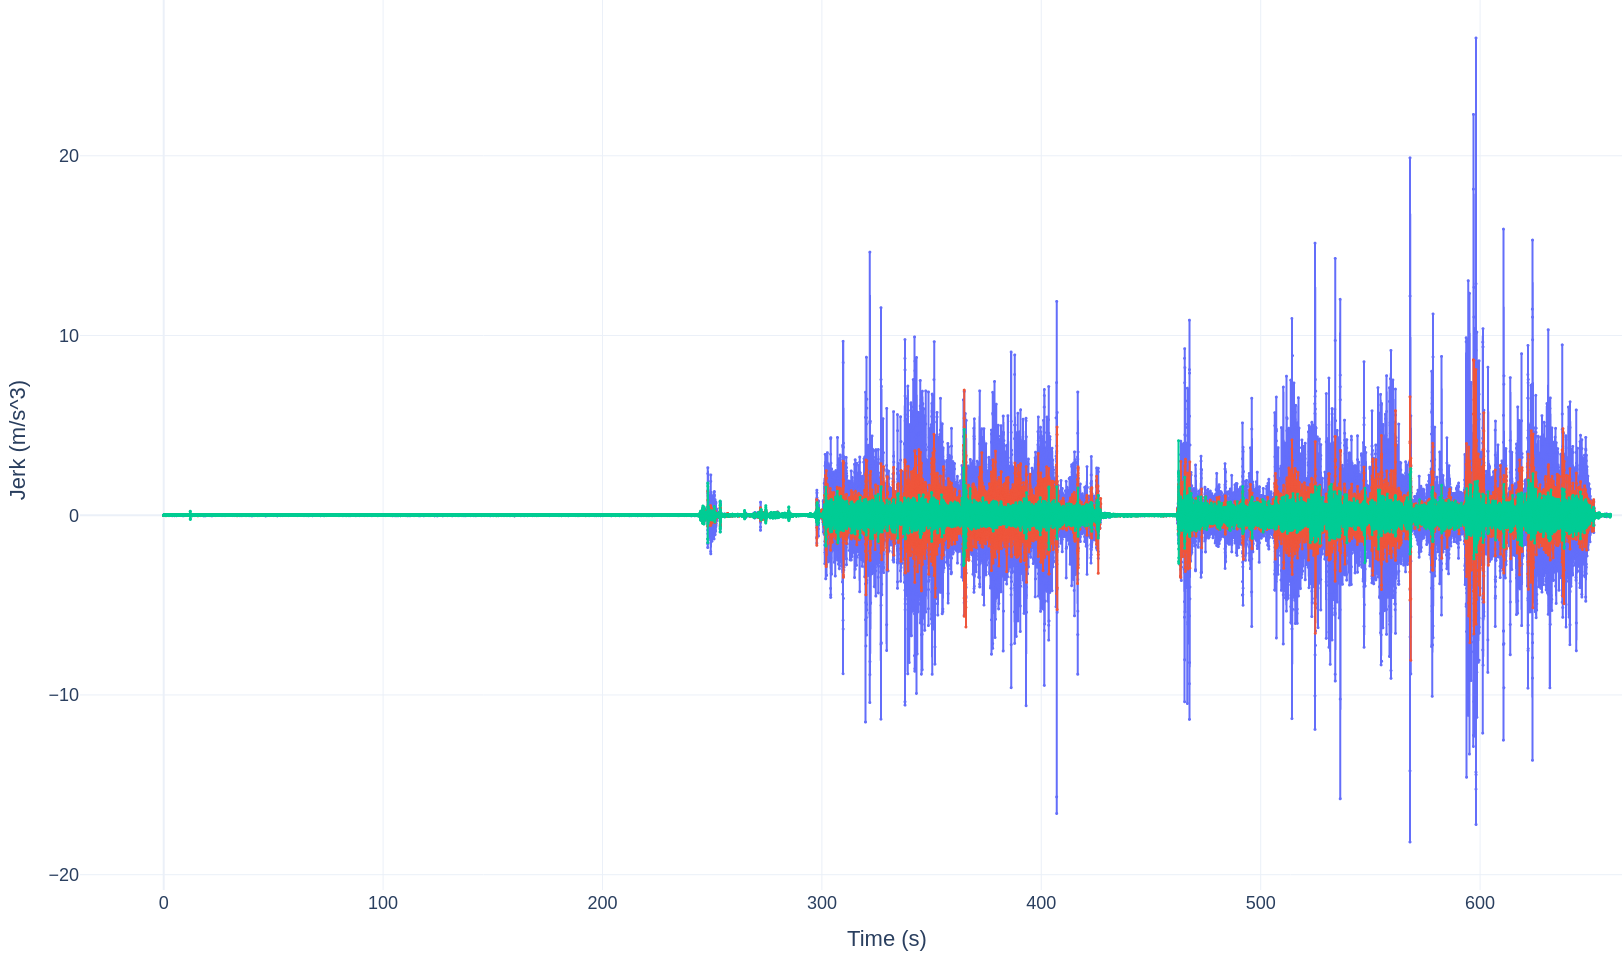
\includegraphics[width=.9\linewidth]{/home/dpaletti/mida_acv/resources/plots/jerk_full_didonato_105.png}
\caption{\label{fig:speed_jessica}Jerk from Didonato's recording}
\end{figure}
\end{frame}
\begin{frame}[label={sec:org84221ee}]{Jerk: two drivers}
\begin{figure}[htbp]
\centering
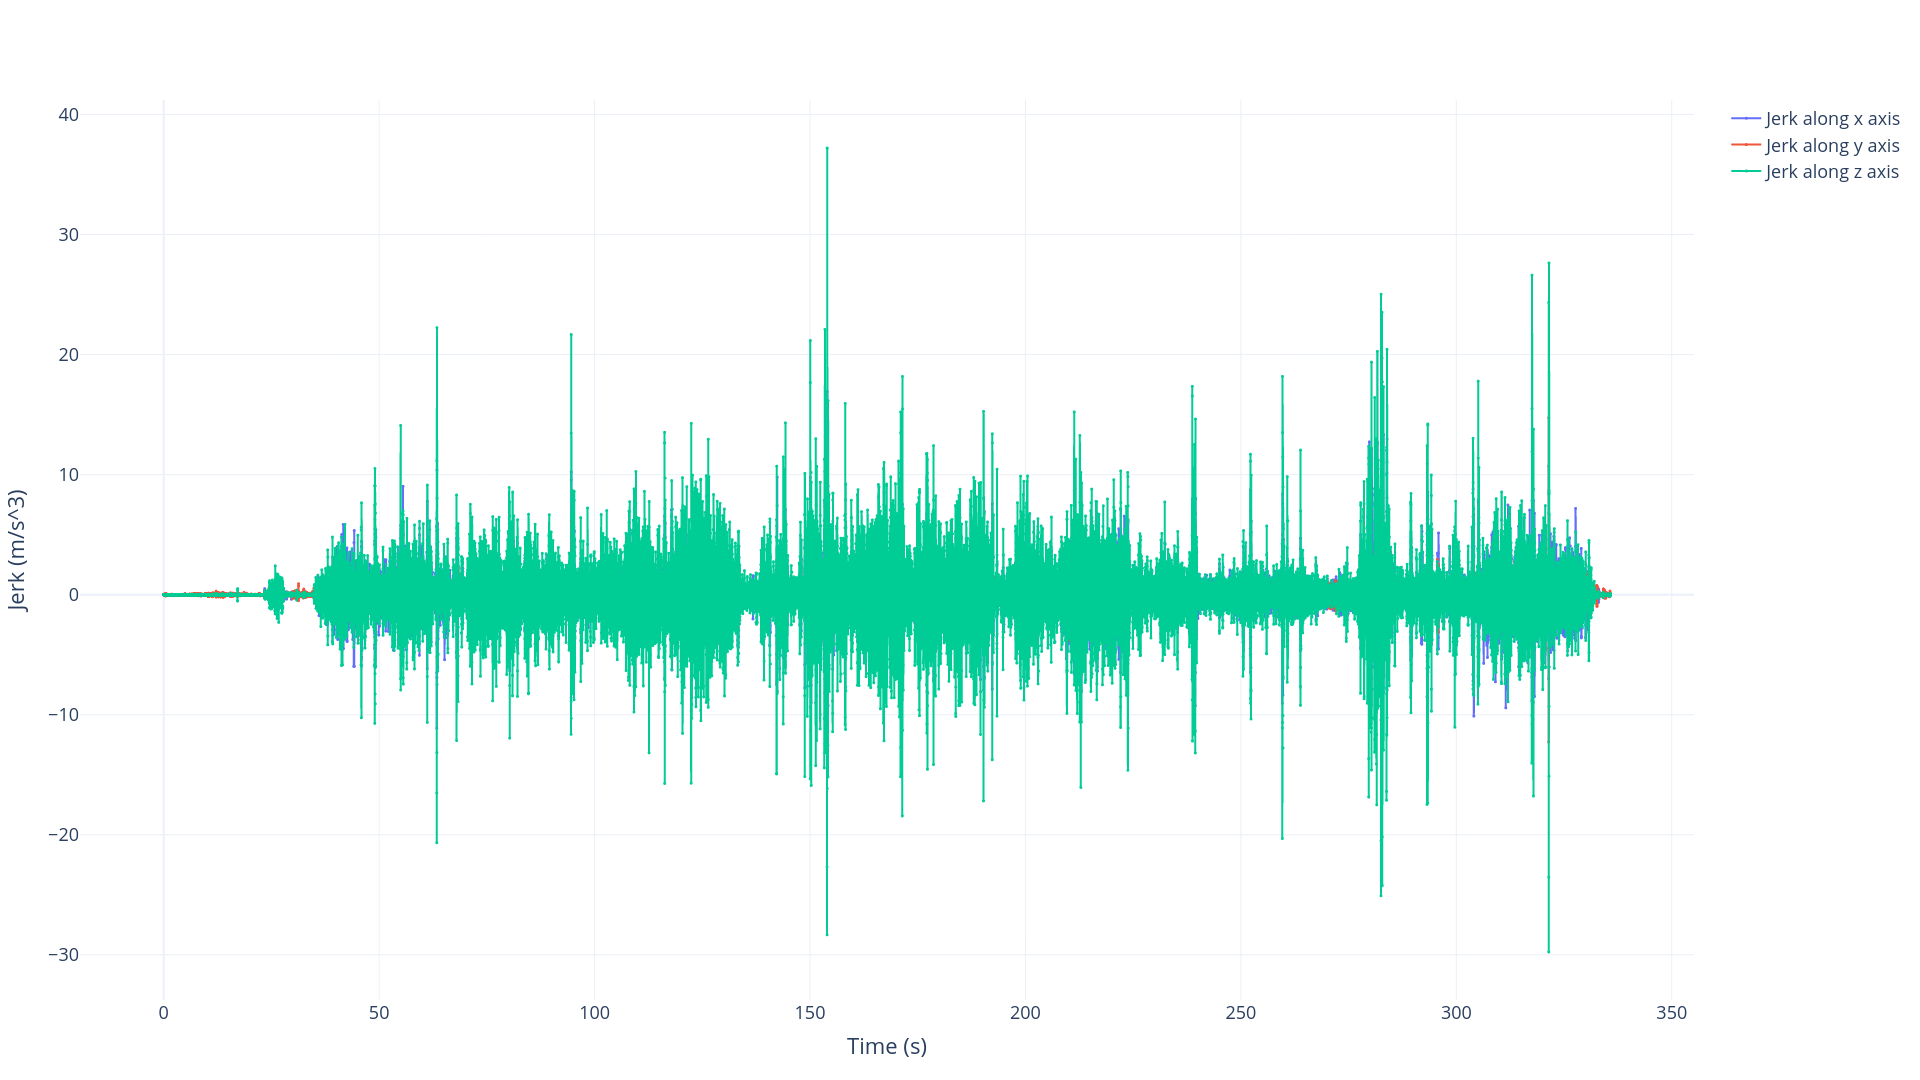
\includegraphics[width=.9\linewidth]{/home/dpaletti/mida_acv/resources/plots/jerk_full_alberto_jessica_108.png}
\caption{\label{fig:speed_alberto_jessica}Jerk from Didonato and Leoni's recording}
\end{figure}
\end{frame}

\begin{frame}[label={sec:orgf3143cb}]{Orientation: one driver, low weight}
\begin{figure}[htbp]
\centering
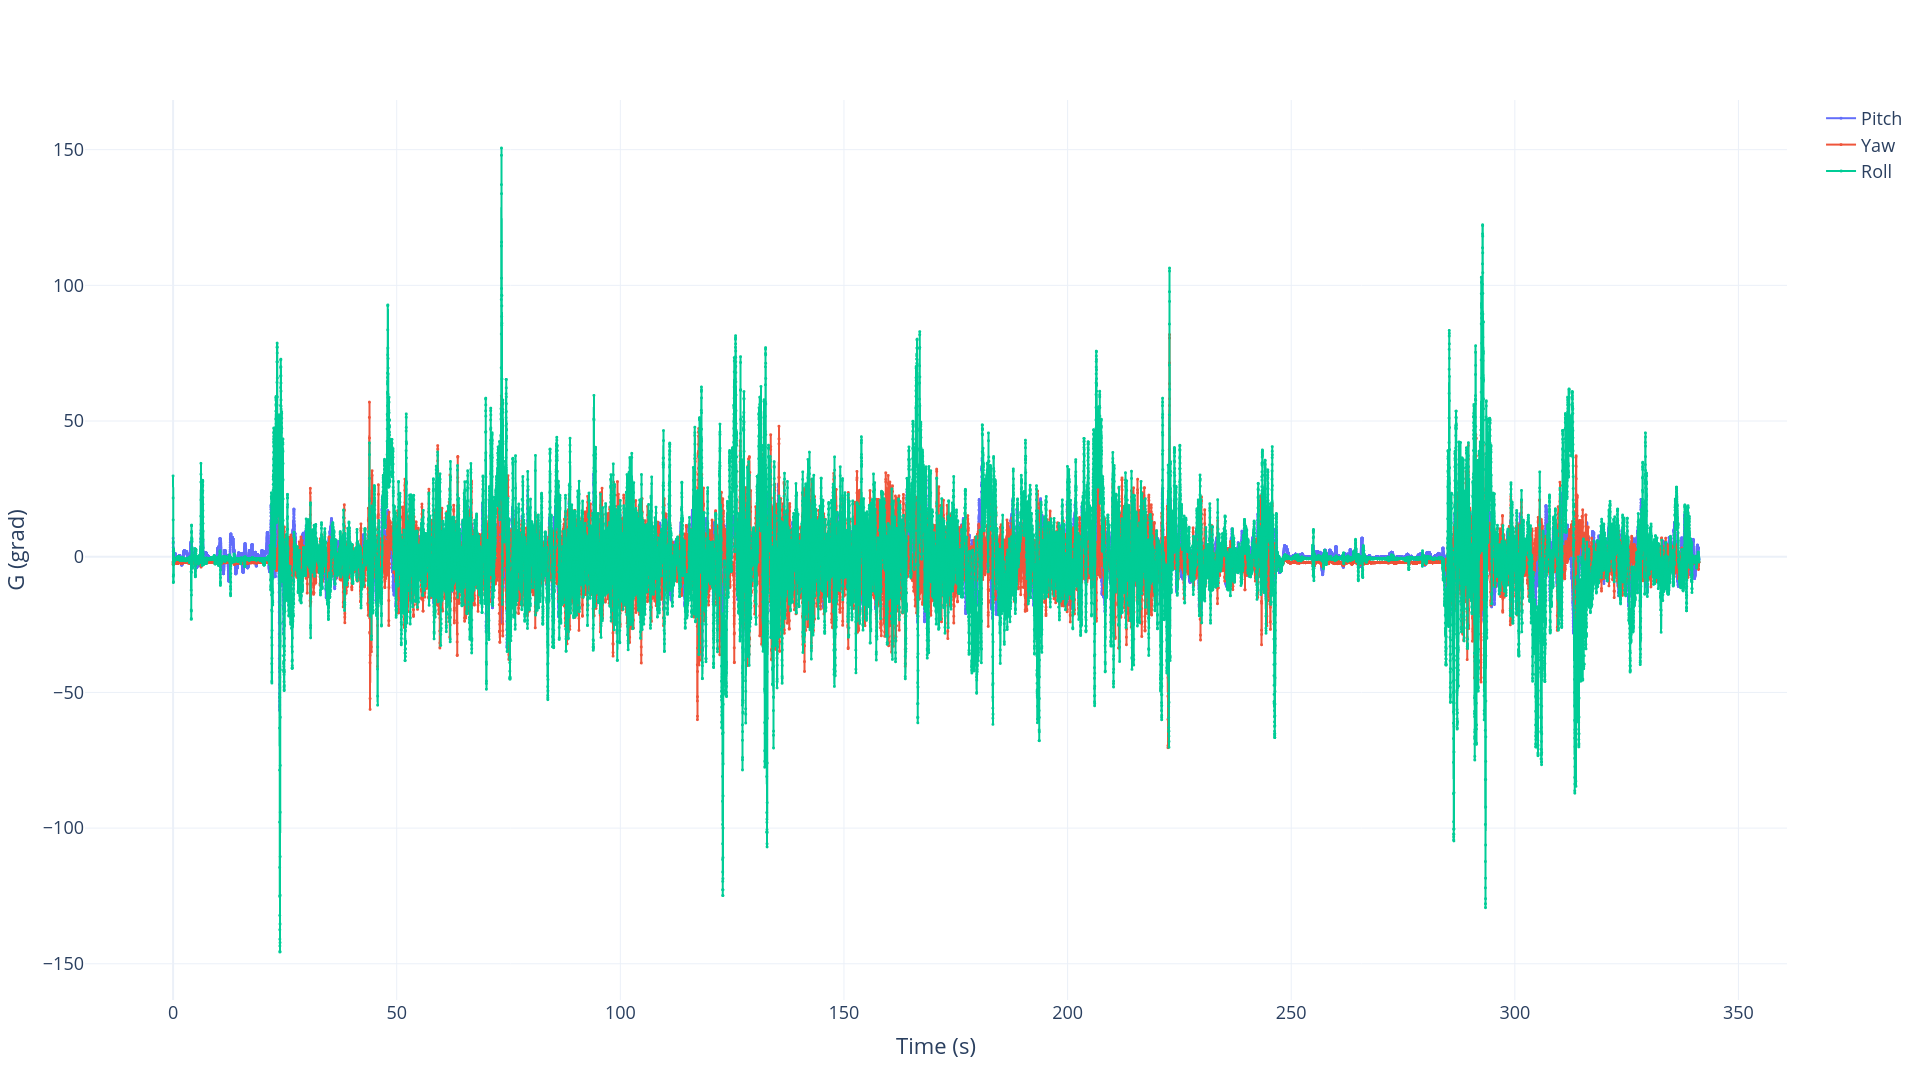
\includegraphics[width=.9\linewidth]{/home/dpaletti/mida_acv/resources/plots/orientation_full_leoni_35.png}
\caption{\label{fig:speed_jessica}Orientation from Leoni's recording}
\end{figure}
\end{frame}
\begin{frame}[label={sec:orge739d22}]{Orientation: one driver, high weight}
\begin{figure}[htbp]
\centering
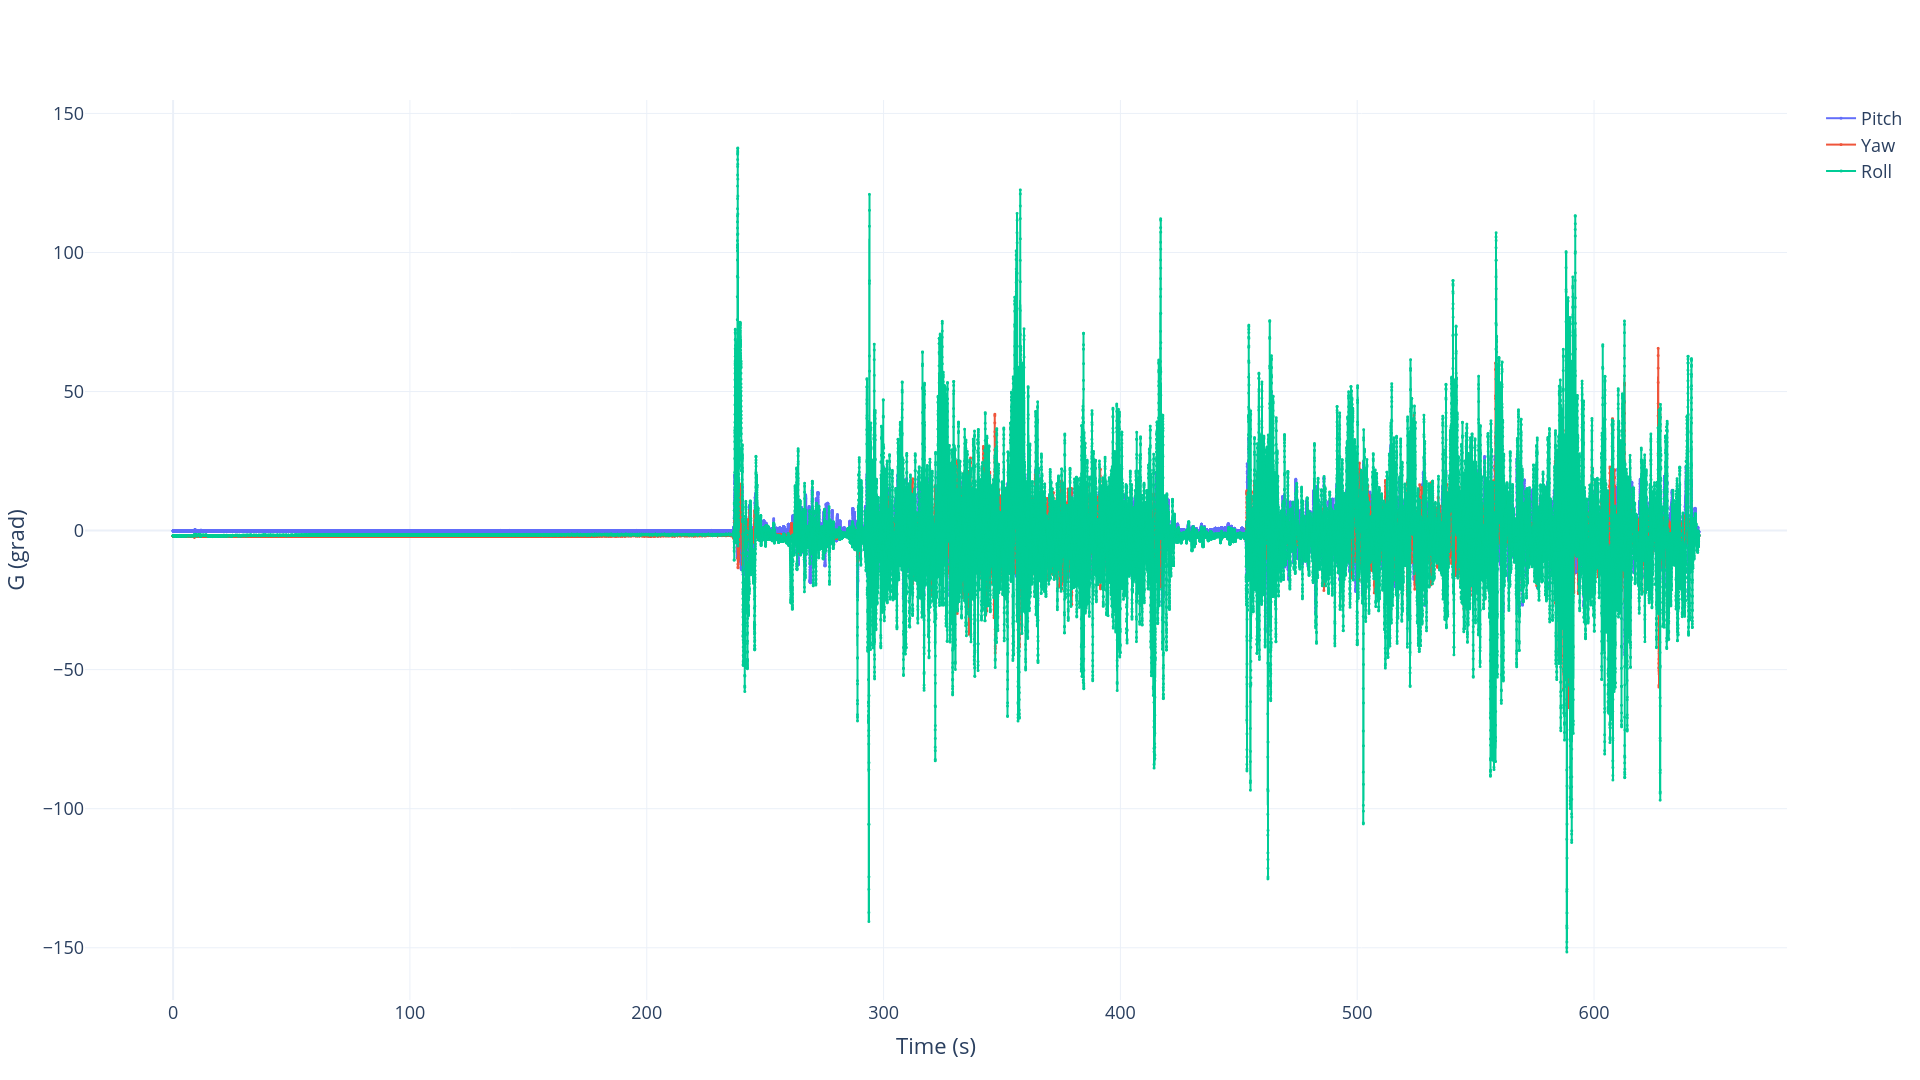
\includegraphics[width=.9\linewidth]{/home/dpaletti/mida_acv/resources/plots/orientation_full_didonato_105.png}
\caption{\label{fig:speed_jessica}Orientation from Didonato's recording}
\end{figure}
\end{frame}
\begin{frame}[label={sec:org6075863}]{Orientation: two drivers}
\begin{figure}[htbp]
\centering
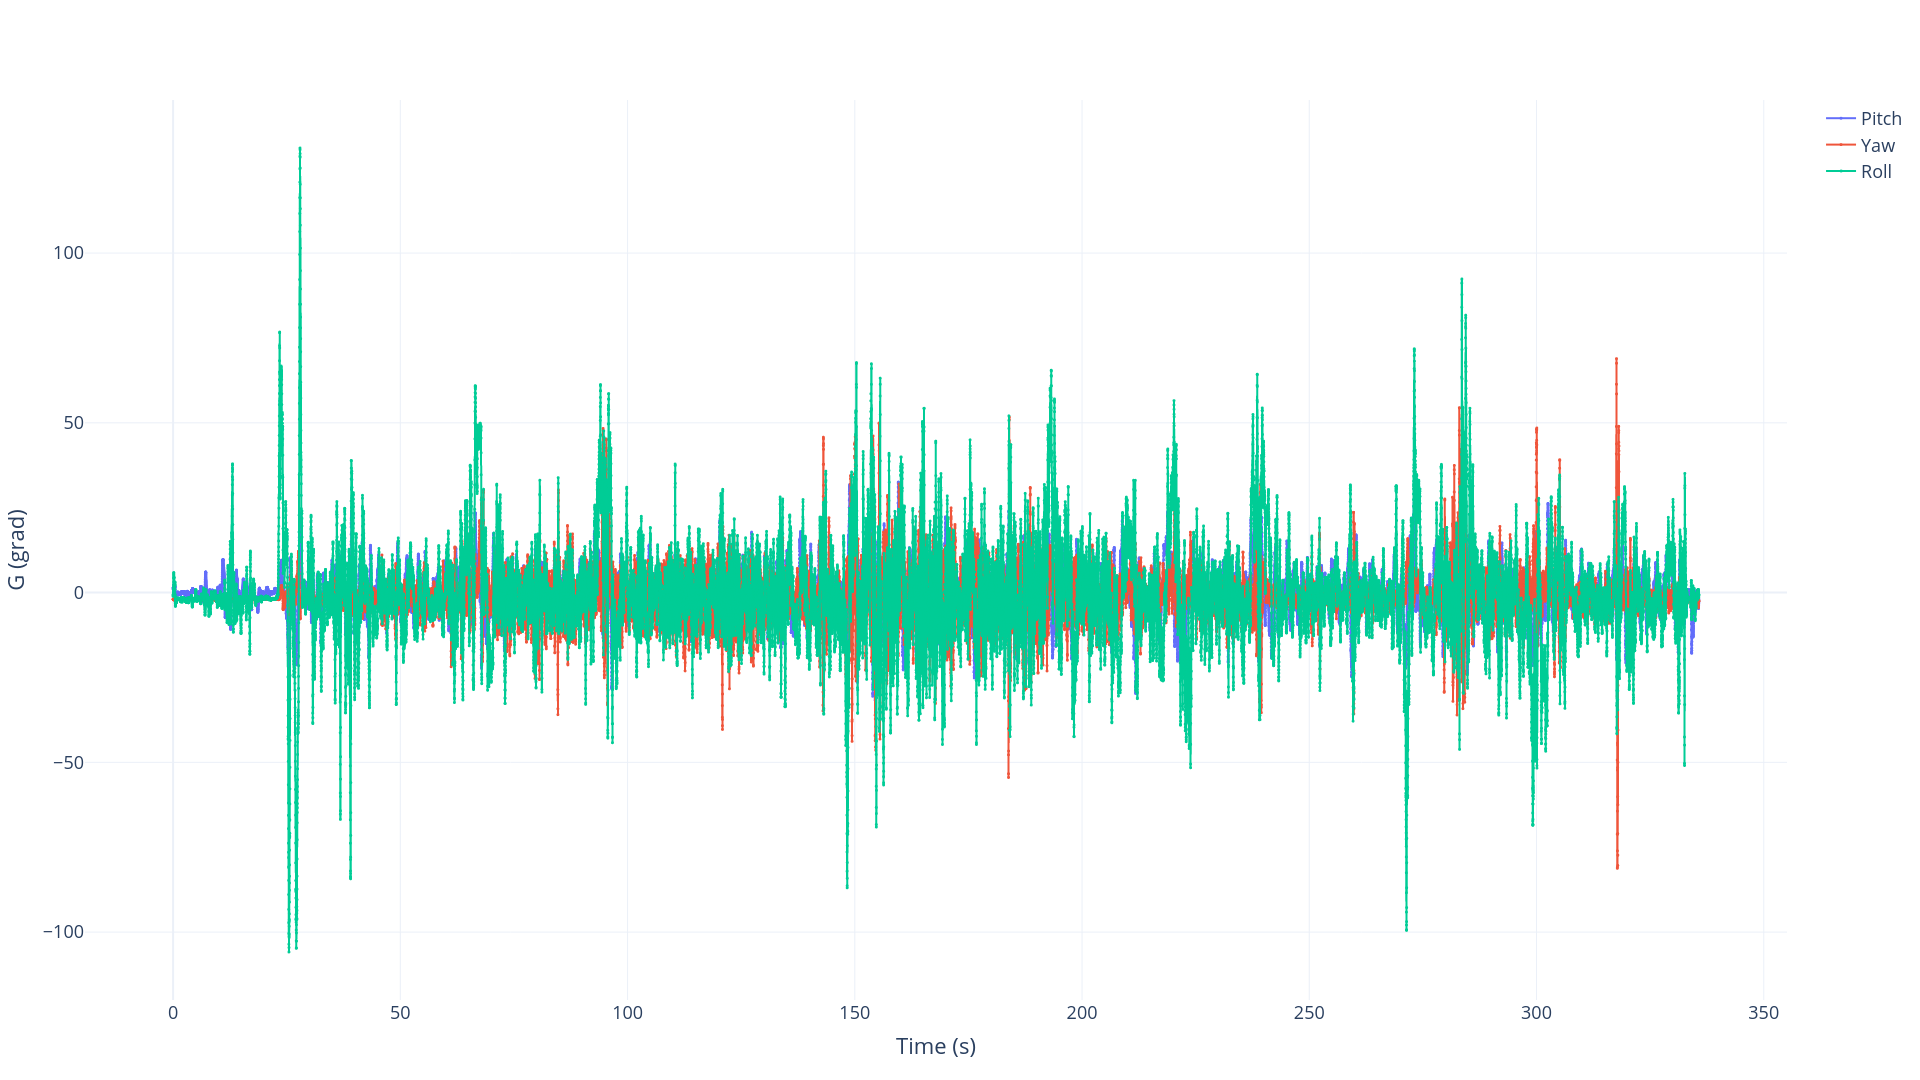
\includegraphics[width=.9\linewidth]{/home/dpaletti/mida_acv/resources/plots/orientation_full_alberto_jessica_108.png}
\caption{\label{fig:speed_alberto_jessica}Orientation from Didonato and Leoni's recording}
\end{figure}
\end{frame}
\section{Data Cleaning}
\label{sec:org4d610e8}
\begin{frame}[label={sec:org4e016e9}]{Removing low speed}
When speed goes lower than 5 km/h the \alert{rider is not on board}, so those points can be removed.
\begin{figure}[htbp]
\centering
\includegraphics[width=.9\linewidth]{/home/dpaletti/Pictures/speed_renzo_jessica_high.png}
\caption{\label{fig:speed_alberto_jessica}Speed from Renzo and Jessica's recording with speed > 5 km/h}
\end{figure}
\end{frame}
\begin{frame}[label={sec:org3f8a7e5}]{Removing low speed: acceleration along x axis}
\begin{figure}[htbp]
\centering
\includegraphics[width=.9\linewidth]{/home/dpaletti/Pictures/ax_renzo_jessica_high.png}
\caption{\label{fig:speed_alberto_jessica}Acceleration along x axis from Renzo and Jessica's recording with corresponging speed > 5 km/h}
\end{figure}
\end{frame}
\begin{frame}[label={sec:org2f07b34}]{Removing low speed: acceleration along y axis}
\begin{figure}[htbp]
\centering
\includegraphics[width=.9\linewidth]{/home/dpaletti/Pictures/ay_renzo_jessica_high.png}
\caption{\label{fig:speed_alberto_jessica}Acceleration along y axis from Renzo and Jessica's recording with corresponging speed > 5 km/h}
\end{figure}
\end{frame}
\begin{frame}[label={sec:org4e1b629}]{Removing low speed: acceleration along y axis}
\begin{figure}[htbp]
\centering
\includegraphics[width=.9\linewidth]{/home/dpaletti/Pictures/az_renzo_jessica_high.png}
\caption{\label{fig:speed_alberto_jessica}Acceleration along y axis from Renzo and Jessica's recording with corresponging speed > 5 km/h}
\end{figure}
\end{frame}
\begin{frame}[label={sec:org45b0299}]{Removing low speed: jerk along x axis}
\begin{figure}[htbp]
\centering
\includegraphics[width=.9\linewidth]{/home/dpaletti/Pictures/jerk_x_renzo_jessica_high.png}
\caption{\label{fig:speed_alberto_jessica}Jerk along x axis from Renzo and Jessica's recording with corresponging speed > 5 km/h}
\end{figure}
\end{frame}
\begin{frame}[label={sec:orgcf035dd}]{Removing low speed: jerk along y axis}
\begin{figure}[htbp]
\centering
\includegraphics[width=.9\linewidth]{/home/dpaletti/Pictures/jerk_y_renzo_jessica_high.png}
\caption{\label{fig:speed_alberto_jessica}Jerk along y axis from Renzo and Jessica's recording with corresponging speed > 5 km/h}
\end{figure}
\end{frame}
\begin{frame}[label={sec:orgcaeba0c}]{Removing low speed: jerk along z axis}
\begin{figure}[htbp]
\centering
\includegraphics[width=.9\linewidth]{/home/dpaletti/Pictures/jerk_z_renzo_jessica_high.png}
\caption{\label{fig:speed_alberto_jessica}Jerk along z axis from Renzo and Jessica's recording with corresponging speed > 5 km/h}
\end{figure}
\end{frame}
\begin{frame}[label={sec:org3f50e55}]{Removing low speed: orientation along x axis}
\begin{figure}[htbp]
\centering
\includegraphics[width=.9\linewidth]{/home/dpaletti/Pictures/gx_renzo_jessica_high.png}
\caption{\label{fig:speed_alberto_jessica}Orientation along x axis from Renzo and Jessica's recording with corresponging speed > 5 km/h}
\end{figure}
\end{frame}
\begin{frame}[label={sec:orgaf52fc7}]{Removing low speed: orientation along y axis}
\begin{figure}[htbp]
\centering
\includegraphics[width=.9\linewidth]{/home/dpaletti/Pictures/gy_renzo_jessica_high.png}
\caption{\label{fig:speed_alberto_jessica}Orientation along y axis from Renzo and Jessica's recording with corresponging speed > 5 km/h}
\end{figure}
\end{frame}
\begin{frame}[label={sec:orgf390641}]{Removing low speed: orientation along z axis}
\begin{figure}[htbp]
\centering
\includegraphics[width=.9\linewidth]{/home/dpaletti/Pictures/gz_renzo_jessica_high.png}
\caption{\label{fig:speed_alberto_jessica}Orientation along z axis from Renzo and Jessica's recording with corresponging speed > 5 km/h}
\end{figure}
\end{frame}
\begin{frame}[label={sec:orgd24d33b}]{Filtering at 1 Hz}
When extracting features in the \alert{time domain} we are not interested in information contained above 1Hz. \newline
Our data is already filtered at 20 Hz.
\begin{figure}[htbp]
\centering
\includegraphics[width=.9\linewidth]{/home/dpaletti/Pictures/speed_renzo_jessica_filtered.png}
\caption{\label{fig:speed_alberto_jessica}Speed filtered at 1 Hz from Renzo and Jessica's recording}
\end{figure}
\end{frame}
\begin{frame}[label={sec:orgecdddb5}]{Filtering at 1 Hz: acceleration along x axis}
\begin{figure}[htbp]
\centering
\includegraphics[width=.9\linewidth]{/home/dpaletti/Pictures/ax_renzo_jessica_filtered.png}
\caption{\label{fig:speed_alberto_jessica}Acceleration along x axis filtered at 1 Hz from Renzo and Jessica's recording}
\end{figure}
\end{frame}
\begin{frame}[label={sec:org00245b3}]{Filtering at 1 Hz: acceleration along y axis}
\begin{figure}[htbp]
\centering
\includegraphics[width=.9\linewidth]{/home/dpaletti/Pictures/ay_renzo_jessica_filtered.png}
\caption{\label{fig:speed_alberto_jessica}Acceleration along y axis filtered at 1 Hz from Renzo and Jessica's recording}
\end{figure}
\end{frame}
\begin{frame}[label={sec:org53a1010}]{Filtering at 1 Hz: acceleration along z axis}
\begin{figure}[htbp]
\centering
\includegraphics[width=.9\linewidth]{/home/dpaletti/Pictures/az_renzo_jessica_filtered.png}
\caption{\label{fig:speed_alberto_jessica}Acceleration along z axis filtered at 1 Hz from Renzo and Jessica's recording}
\end{figure}
\end{frame}
\begin{frame}[label={sec:org5a3c044}]{Filtering at 1 Hz: jerk along x axis}
\begin{figure}[htbp]
\centering
\includegraphics[width=.9\linewidth]{/home/dpaletti/Pictures/jerk_x_renzo_jessica_filtered.png}
\caption{\label{fig:speed_alberto_jessica}Jerk along x axis filtered at 1 Hz from Renzo and Jessica's recording}
\end{figure}
\end{frame}
\begin{frame}[label={sec:org5e1326f}]{Filtering at 1 Hz: jerk along y axis}
\begin{figure}[htbp]
\centering
\includegraphics[width=.9\linewidth]{/home/dpaletti/Pictures/jerk_y_renzo_jessica_filtered.png}
\caption{\label{fig:speed_alberto_jessica}Jerk along y axis filtered at 1 Hz from Renzo and Jessica's recording}
\end{figure}
\end{frame}
\begin{frame}[label={sec:org0140e8e}]{Filtering at 1 Hz: jerk along z axis}
\begin{figure}[htbp]
\centering
\includegraphics[width=.9\linewidth]{/home/dpaletti/Pictures/jerk_z_renzo_jessica_filtered.png}
\caption{\label{fig:speed_alberto_jessica}Jerk along z axis filtered at 1 Hz from Renzo and Jessica's recording}
\end{figure}
\end{frame}
\begin{frame}[label={sec:orgf23e204}]{Filtering at 1 Hz: orientation along x axis}
\begin{figure}[htbp]
\centering
\includegraphics[width=.9\linewidth]{/home/dpaletti/Pictures/gx_renzo_jessica_filtered.png}
\caption{\label{fig:speed_alberto_jessica}Orientation along x axis filtered at 1 Hz from Renzo and Jessica's recording}
\end{figure}
\end{frame}
\begin{frame}[label={sec:orgdfb739b}]{Filtering at 1 Hz: orientation along y axis}
\begin{figure}[htbp]
\centering
\includegraphics[width=.9\linewidth]{/home/dpaletti/Pictures/gy_renzo_jessica_filtered.png}
\caption{\label{fig:speed_alberto_jessica}Orientation along y axis filtered at 1 Hz from Renzo and Jessica's recording}
\end{figure}
\end{frame}
\begin{frame}[label={sec:org8eea099}]{Filtering at 1 Hz: orientation along z axis}
\begin{figure}[htbp]
\centering
\includegraphics[width=.9\linewidth]{/home/dpaletti/Pictures/gz_renzo_jessica_filtered.png}
\caption{\label{fig:speed_alberto_jessica}Orientation along z axis filtered at 1 Hz from Renzo and Jessica's recording}
\end{figure}
\end{frame}
\section{Data Selection}
\label{sec:orgaf7c486}
\begin{frame}[label={sec:org4e7e77d}]{Path simplification}
\alert{Ramer-Douglas-Pecker} algorithm can be used to \alert{downsample} input data to remove redundant points on straight lines. \newline
The only algorithm parameter is \alert{epsilon}, the lower the more points are retained. \newline
We decided non to use this approach because in the \alert{frequency} domain a lot of relevant \alert{information is lost}.
\begin{figure}[htbp]
\centering
\includegraphics[width=.9\linewidth]{/home/dpaletti/Pictures/path_jessica_alberto_simplified.png}
\caption{\label{fig:speed_alberto_jessica}Simplified Path of Jessica and Alberto's recording (epsilon=1e-6)}
\end{figure}
\end{frame}
\begin{frame}[label={sec:orgf39a95e}]{Path simplification time domain: 0.7\% samples}
\begin{figure}[htbp]
\centering
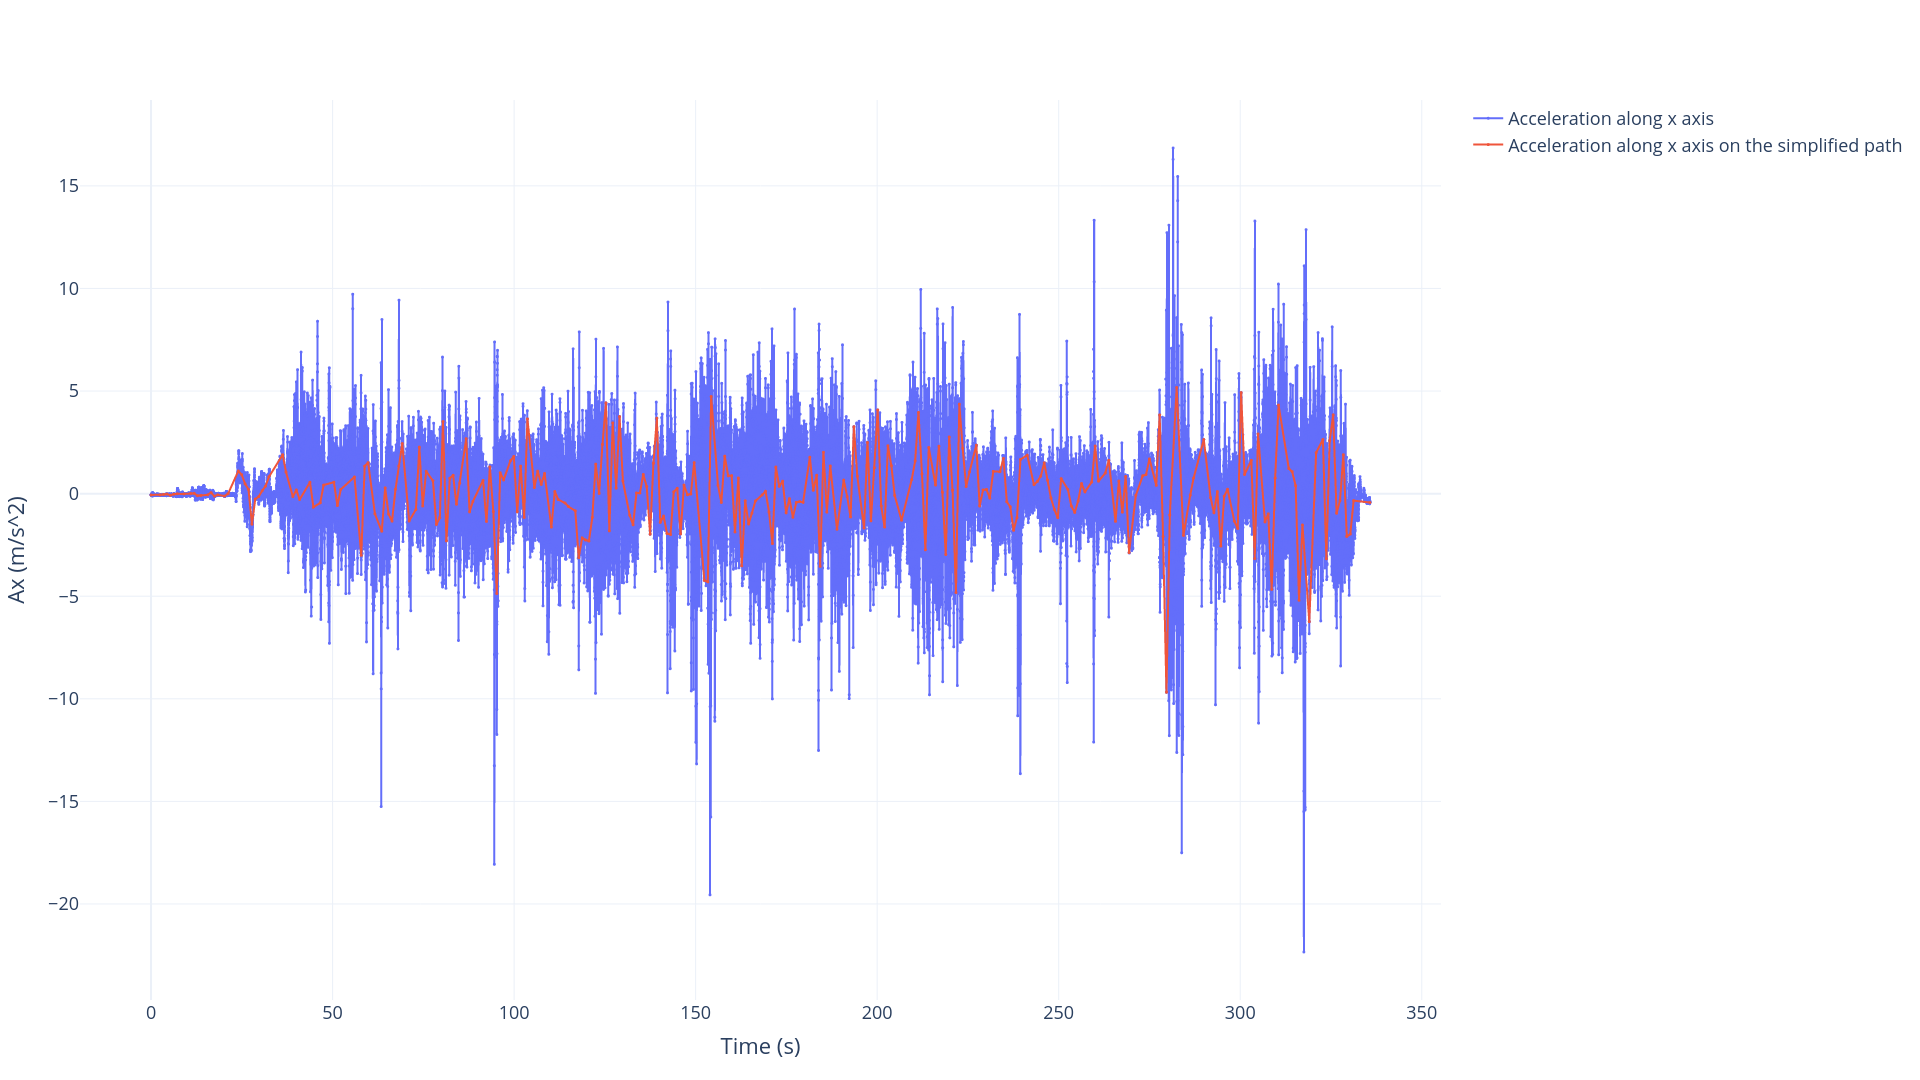
\includegraphics[width=.9\linewidth]{/home/dpaletti/mida_acv/resources/plots/Accelerationx_alberto_jessica_108_0.000001.png}
\caption{Simplified Acceleration of Jessica and Alberto's recording (epsilon=1e-6, 6000/768000 samples on the whole stem dataset)}
\end{figure}
\end{frame}
\begin{frame}[label={sec:org4a62625}]{Path simplification frequency domain: 20\% samples}
\begin{figure}[htbp]
\centering
\includegraphics[width=.9\linewidth]{/home/dpaletti/Pictures/ax_spectrum_1e-14.png}
\caption{Simplified Acceleration of Jessica and Alberto's recording (epsilon=1e-14)}
\end{figure}
\end{frame}
\begin{frame}[label={sec:orgf2f72eb}]{Path simplification frequency domain: 80\% samples}
\begin{figure}[htbp]
\centering
\includegraphics[width=.9\linewidth]{/home/dpaletti/Pictures/ax_1e-16.png}
\caption{Simplified Acceleration of Jessica and Alberto's recording (epsilon=1e-16)}
\end{figure}
\end{frame}

\begin{frame}[label={sec:org8d149a6}]{Downsampling}
Regular downsampling, taking \alert{one every two samples}, allows to halve the original sampling frequency while it does not effect too badly the signal in the frequency domain.
\end{frame}
\section{Feature Engineering}
\label{sec:org6f36c1c}
\begin{frame}[label={sec:orga6b5e57}]{Overview}
\begin{center}
\includegraphics[width=.9\linewidth]{/home/dpaletti/Pictures/feature_extraction_process.png}
\end{center}
\end{frame}
\begin{frame}[label={sec:org6aeaaee}]{Feature extraction}
\begin{columns}
\begin{column}[t]{0.5\columnwidth}
We employ a prominent python library for time series analysis: \alert{tsfresh}. \newline
Feature extraction can be carried out for each measurement through the tools provided by the library. \newline
Extracted features:
\begin{itemize}
\item mean
\item variance
\item maximum
\item minimum
\item root mean square
\item fast fourier transform area
\end{itemize}
\end{column}
\begin{column}[t]{0.5\columnwidth}
\begin{center}
\includegraphics[width=.9\linewidth]{/home/dpaletti/Pictures/tsfresh.png}
\end{center}
\end{column}
\end{columns}
\end{frame}
\begin{frame}[label={sec:org4ec0940}]{Feature Selection: Significance}
Each feature vector is individually and independently evaluated with respect to its \alert{significance for predicting the target} under investigation.  \newline
\alert{Statistical tests} employed:
\begin{itemize}
\item Kolmogorov-Smirnov: binary valued feature (confidence) and real valued target (weight class)
\item Kendall’s tau: real feature and real valued target
\item Two-sided univariate Fisher test: binary feature and binary valued target (two riders detection)
\item Mann-Whitney U: real valued feature and binary valued target
\end{itemize}
\end{frame}
\begin{frame}[label={sec:org9dd9330}]{Feature Selection: p-value evaluation}
Once the tests are applied we get a \alert{vector of p-values} quantifying the importance of each feature. \newline
\alert{Benjamini-Yekutieli} procedure is applied to decide which feature to keep
\end{frame}
\section{Roadmap}
\label{sec:orgecfa351}
\begin{frame}[label={sec:orgcb24b3b}]{Roadmap}
\begin{center}
\includegraphics[width=.9\linewidth]{/home/dpaletti/Pictures/roadmap.png}
\end{center}
\end{frame}
\end{document}
